\documentclass[a4paper,12pt]{report}

\usepackage{xeCJK}
\setCJKmainfont{Songti SC}
\usepackage{fullpage}
\usepackage{url}
\usepackage{setspace}
\onehalfspacing
\usepackage{graphicx}
\usepackage{amsmath}
\usepackage{minted}

\usepackage[backend=biber,style=numeric-comp]{biblatex}
\bibliography{essay.bib}
\usepackage[nottoc]{tocbibind}

\begin{document}

\title{生命游戏与加密算法}
\author{
	信息科学技术学院\\
	计算机科学与技术\\
	赵睿哲\\
	1200012778}
\maketitle

\begin{abstract}

\end{abstract}

\tableofcontents

\chapter{生命游戏概述}

生命游戏(Game of Life)由英国剑桥大学的数学家康威(John Horton Conway)于1970年提出\footfullcite{gardner1970mathematical},是一个特殊的细胞自动机(Cellular Automaton,简称CA)。从一个随机的初始状态出发,该细胞自动机会随时间一步步演化,并根据初始状态的不同有完全不一样的特征。根据理论与实验可以发现,生命游戏在某些条件下具有显著的混沌特征。本章首先介绍细胞自动机的基本概念,进而分析并实现了生命游戏的基本版本。下一章对生命游戏的混沌性质进行具体分析。

\section{细胞自动机}

细胞自动机的概念源自于冯·诺依曼 (John von Neumann) 对自我复制系统 (Self-replication systems) 的研究。冯·诺依曼想要模拟生命的自我复制过程,通过借鉴了乌拉姆 (Stanislaw Ulam) 所设计的晶格模型 (Lattice model),于1940年代设计了细胞自动机的原始样态\footfullcite{schiff2011cellular}。

细胞自动机是是一个离散的系统,其离散性体现在:1) 每个细胞是规则的网格单元,通过明确的边界分隔,网格可以组成一维、二维或者是更高维的欧氏空间;2) 每个细胞具有有限个数的状态,比如“存活”或者“死亡”;3) 细胞自动机的演化过程是时间离散的,可以用离散的时间步进行模拟。

细胞自动机的演化依据确定的规则,演化规则一般与细胞的状态与其邻居的状态共同决定。细胞的邻居定义不固定,一般情况下,一维的细胞自动机取一定半径范围内的细胞作为邻居,二维细胞自动机取上下、左右以及四个对角线方向上的细胞作为邻居 (即摩尔邻居,Moore Neighbourhood,如图\ref{fig:moore})。

\begin{figure}[!ht]
\centering
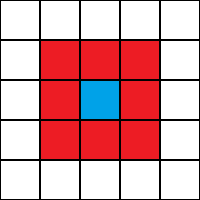
\includegraphics[width=0.3\textwidth]{images/CA-Moore.png}
\caption{摩尔邻居的样例,图例为二维平面细胞自动机,红色网格为邻居细胞,蓝色网格为目标细胞}
\label{fig:moore}
\end{figure}

下一节具体介绍生命游戏这一种细胞自动机的实现。

\section{生命游戏}\label{sec:gol}

生命游戏是一种特殊的细胞自动机,它的定义如下:首先,生命游戏是个二维的细胞自动机,邻居的定义与摩尔邻居相同;其次,细胞状态有“存活”和“死亡”两种,细胞的下一个状态由当前状态和邻居状态共同决定。生命游戏的演化规则如下:

令$S_{i,j}^t \in \{ 0, 1 \}$为时刻$t$时位于坐标$(i,j)$的细胞状态:取值为0,表示“死亡”;或者1,表示“存活”。下一个状态$S_{i,j}^{t+1}$取决于当前状态和邻居的状态之和,令邻居状态值之和为$\overline{S}_{i,j}$,即:
$$
\overline{S}_{i,j} = \sum_{x=i-1}^{i+1} \sum_{y=j-1}^{j+1} S_{x,y}^t 
$$

则转换函数为:
\begin{equation}\label{eq:mapping}
S_{i,j}^{t+1} = f(S_{i,j}^t) = 
\begin{cases}
0 & \texttt{if } S_{i,j}^t = 0 \wedge  \overline{S}_{i,j} \neq 3 \\
  & \texttt{or } S_{i,j}^t = 1 \wedge (\overline{S}_{i,j} \leq 1 \vee \overline{S}_{i,j} \geq 4) \\
1 & \texttt{if } S_{i,j}^t = 0 \wedge \overline{S}_{i,j} = 3 \\
  & \texttt{or } S_{i,j}^t = 1 \wedge 2 \leq \overline{S}_{i,j} \leq 3 \\
\end{cases}
\end{equation}

从生态系统的角度理解,$\overline{S}_{i,j}$的值可以衡量一个细胞的邻居范围内的“拥挤”情况:如果当前细胞的状态是“存活”,并且周围过于拥挤的话,那么该细胞就会“死亡”;同时$\overline{S}_{i,j}$值过小,代表周围“存活”细胞太少,那么当前细胞也会因为缺少“同伴”而“死亡”。

\section{生命游戏的实现}

本文使用Python语言实现了一个简单的生命游戏小程序,如代码\ref{lst:gol}所示
\footnote{代码开源于\url{https://github.com/kumasento/gameoflife}}。类Life中保存了当前时刻的每个细胞的状态,在\texttt{state}中。细胞的状态为一个二维数组,每一个元素取值为0或者1,初始化时为随机生成。
\singlespacing
\begin{listing}[!ht]
\inputminted[
	breaklines,
	mathescape,
	linenos,
	numbersep=5pt,
	fontsize=\footnotesize]{py}{codes/life.py}
\label{lst:gol}
\caption{生命游戏的简单Python实现}
\end{listing}
\onehalfspacing

此外,上述代码使用了卷积(行15)进行计算优化。\texttt{w}为卷积权值矩阵,对任意一个细胞,周围邻居的权值均为1,自己的权值为10,这样就可以把\ref{eq:mapping}中的映射函数变为一个简单的转换表。具体来说,该转换表的输入取值从0到18,只有取值为3(对应于\ref{eq:mapping}的第三行条件)或者取值为12、13(对应于\ref{eq:mapping}的第四行条件)才能让状态在下一步转换为“存活”,即1。

\begin{figure}[!ht]
	\centering
	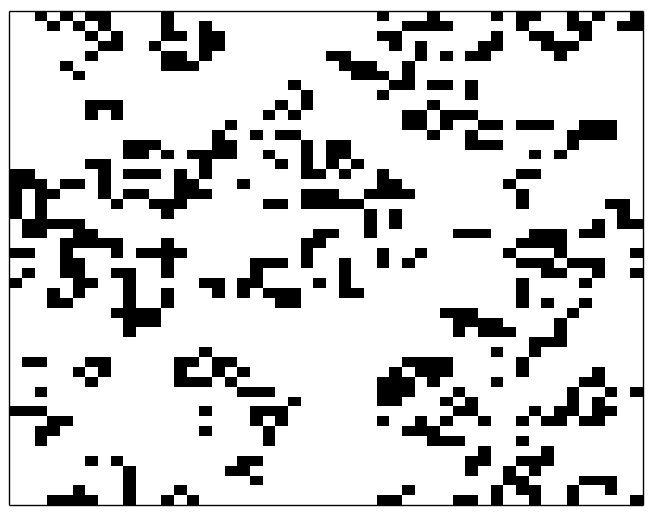
\includegraphics[width=0.4\textwidth]{images/gol.png}
	\label{fig:gol}
	\caption{50 X 50的生命游戏的演化阶段之一}
\end{figure}

生命游戏的展示使用了\texttt{matplotlib}作图函数库来实现,制作一个二维坐标图,如果对应的坐标细胞为存活则染色为黑色,否则为背景色(白色)。系统的演化的动画效果通过不断刷新图像来实现。最后的演示效果图\ref{fig:gol}。

在使用上述代码进行演示时,会发现生命游戏随着初始结构的不同,会有完全不一样的演化结果,可以说体现了一定的混沌性质。下一章对生命游戏的混沌性质进行具体的分析。

\chapter{生命游戏的性质}

生命游戏的演化结果对初始状态十分敏感,演化的形态多种多样。本章首先给出几种生命游戏常见的形态,之后进行演化性质进行理论推导。

\section{驱动力与耗散力}

正如第\ref{sec:gol}节对生命游戏的分析,生命游戏可以看做是对生态系统的某种程度上的模拟。整个系统的演化取决于驱动力和耗散力之间的相互作用。本论文认为生命游戏的驱动力是令细胞从“死亡”到“存活”或者保持“存活”状态的力,而耗散力则是令细胞从“存活”走向“死亡”的力。更具体一些,即为映射\ref{eq:mapping}中的两种结果对应的条件。令下一时刻状态为0的条件都是系统的耗散力,令下一时刻状态为1的条件都是系统的驱动力。

\section{演化过程分析}

正如前述,生命游戏有各种不同的演化种类,有的经过简单的几步即可收敛为静止,有的会进行周期性的转变,有的甚至进入混沌状态。

为了简化分析过程,本章以一个$N \times N$的有限网格作为分析对象。在该网格边界的细胞,可以认为它们的值为0。这种做法会导致位于边上的细胞更容易存活,位于角上的细胞更容易死亡。

通过简单的推理可以发现,当$N$的取值比较小时,整个生命游戏系统对应的映射函数也比较简单,应该比较容易收敛到定常解或者进入周期的变化。当$N$取值较大时,在有限的演化步中很可能无法收敛,处于混沌状态。因此本节接下来按照不同的$N$的尺度进行分析,对小尺度的$N$\textbf{定量}分析定常解跟周期解的形态,对大尺度的$N$则进行定性的分析。需要注意的是,即使是小尺度的$N$,初始化状态也有$2^{N^2}$种,当$N=5$时已经有$33554432$种情况。因此对小尺度的分析只针对$2 \leq N \leq 5$。同时,这么多种情况很难使用手工推导和识别,因此使用程序进行分析。

如何使用程序进行分析?首先,该程序的功能是枚举所有的初始状态,并计算其最终的收敛结果。因此最关键的是如何判断生命游戏是否收敛。本论文中使用的策略如下:给定迭代次数\texttt{max\_iter},迭代完成后,从最后一个迭代结果出发判断是否满足从$1$开始的周期数。因此能找到的周期上界是$\lfloor \mathtt{max\_iter} \rfloor$,如果系统的周期数比该数值高或者无法得到周期解,都判断为混沌状态。该算法的时间复杂度为$O(2^{N^2} \times N^2 \times \mathtt{max\_iter})$,即对所有初始状态($2^{N^2}$个)计算迭代$\mathtt{max\_iter}$次的结果,每次迭代的复杂度与卷积计算在一个数量级内。

同时,该程序使用\texttt{matplotlib}库生成定常解和周期解的示例图,方便识别规律和验证。此外,使用\texttt{multiprocessing}库对计算进行并行加速,在16核的Intel服务器上,原先需要几天才能算完的$N=5$的情况,现在只需要5.8个小时即可计算完毕。

\subsection{定常解与周期解}

对于小尺度的生命游戏收敛结果的统计如下::
\begin{table}[!ht]
\centering
\begin{tabular}{|l|l|l|l|l|}
\hline
周期数 & $N=2$ & $N=3$ & $N=4$ & $N=5$ \\ \hline
1      & 16    & 510   & 62976 & 30466005 \\ \hline
2      & 0     & 2     & 2512  & 2606499 \\ \hline
3      & 0     & 0     & 48    & 0       \\ \hline
4      & 0     & 0     & 0     & 375176  \\ \hline
5      & 0     & 0     & 0     & 80      \\ \hline
8      & 0     & 0     & 0     & 27072   \\ \hline
12     & 0     & 0     & 0     & 79600   \\ \hline
\end{tabular}
\label{table:stats}
\caption{对小尺度的生命游戏的收敛结果的统计}
\end{table}

通过上述统计结果可以得到的结论如下:

首先,$N=2$与$N=3$非常容易收敛,这是因为可以变化的细胞太少的原因,很容易系统就只剩下处于稳定状态的定常解或者周期解。$N=3$的周期解只有周期为2的情况,并且只有如下一种模式:

\begin{figure}[!ht]
\centering
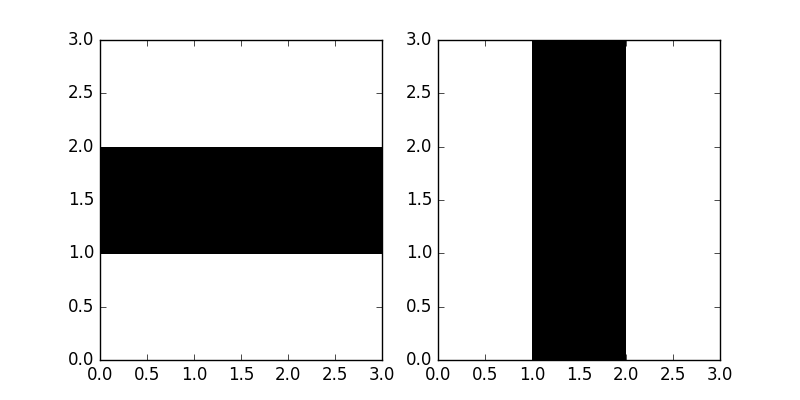
\includegraphics[width=0.5\textwidth]{images/img32.png}
\label{fig:n3}
\caption{$N=3$时出现的周期2模式}
\end{figure}

其次,对于$N=4$或$N=5$的情况,在周期2的时候也重复了图\ref{fig:n3}的模式。但对于其他的周期数而言,得到的模式就比较难以发现了,比如$N=5$的周期数为12的模式之一(如图\ref{fig:n5})。

\begin{figure}[!ht]
\centering
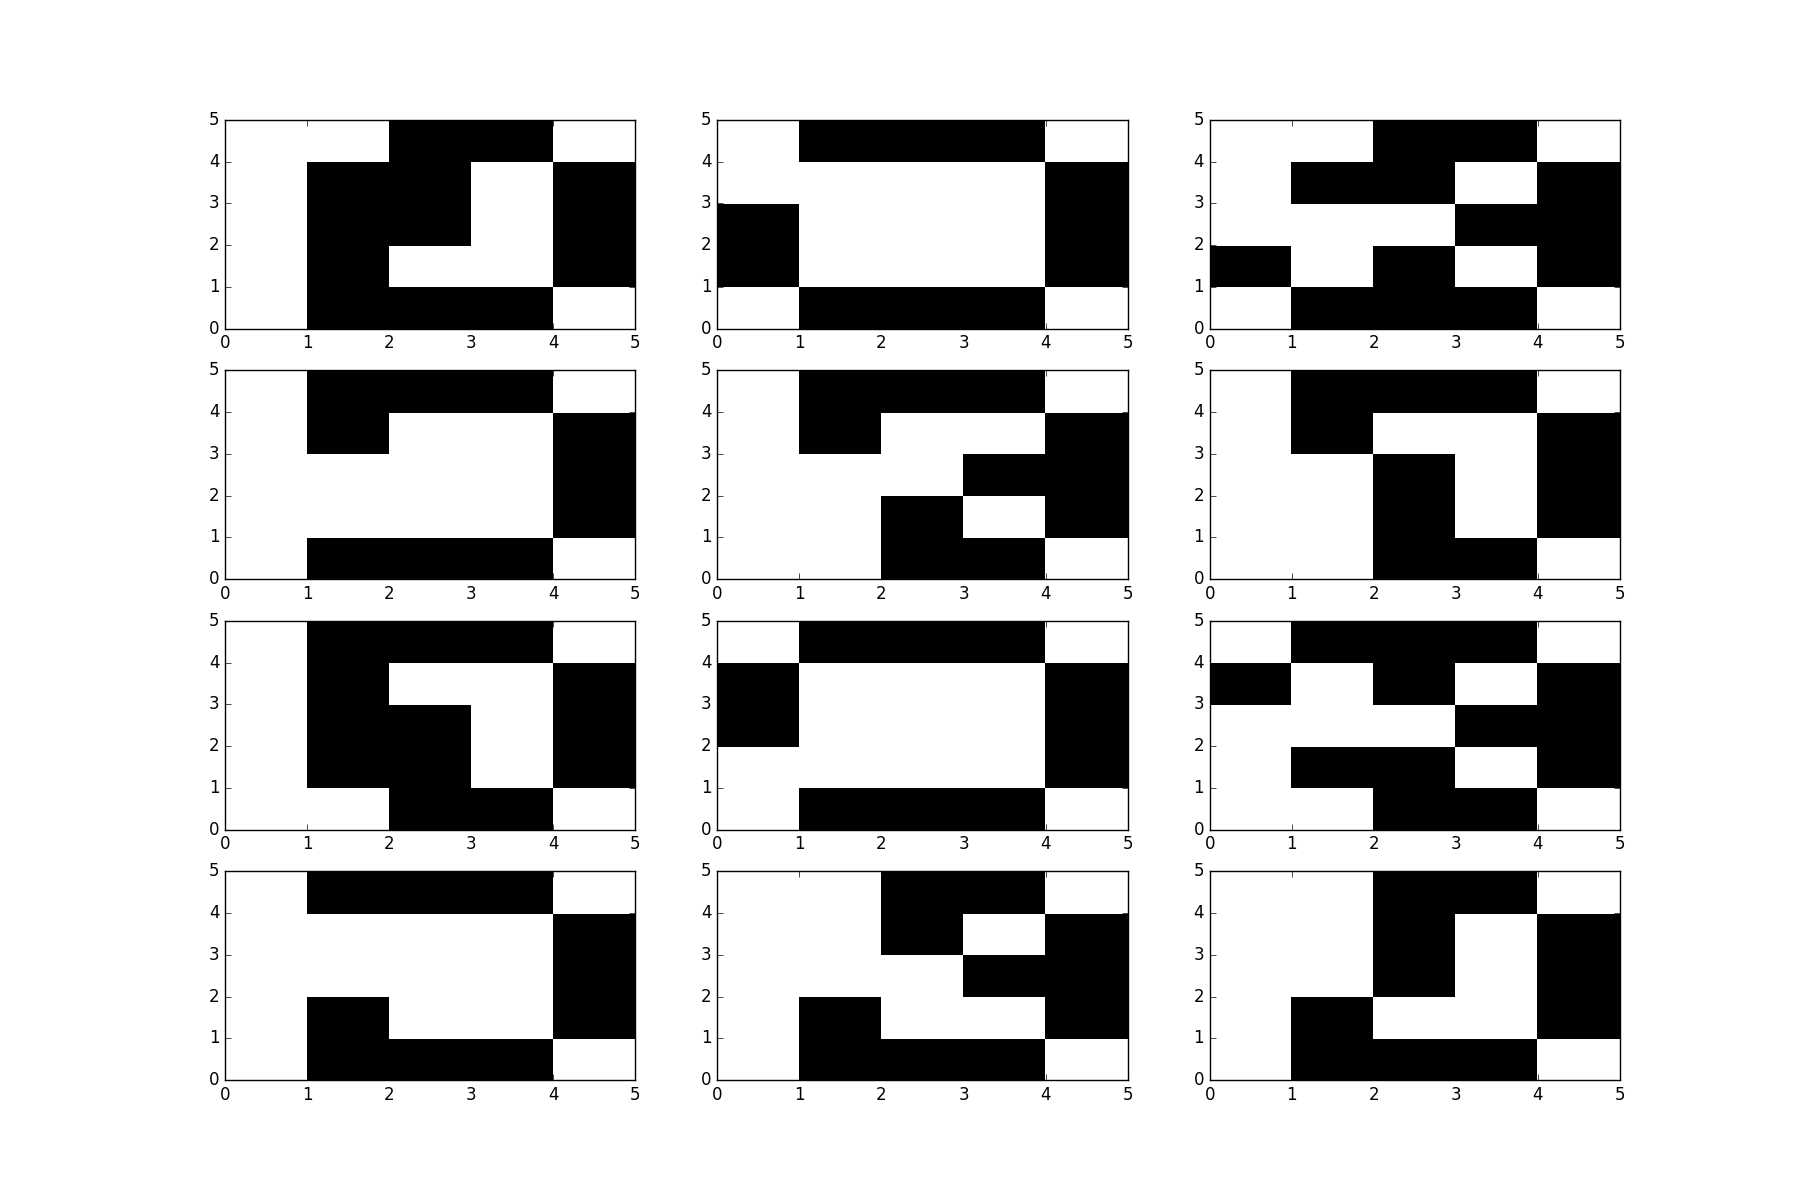
\includegraphics[width=0.8\textwidth]{images/img512.png}
\label{fig:n5}
\caption{$N=5$时的一种周期数为12的模式}
\end{figure}

总之,随着生命游戏的尺度越来越大,产生的模式越来越复杂。可以看出,从$N=2$开始,周期解的个数占比越来越多,同时周期数也越来越大。可以预计,当$N$取值达到一定规模时,很可能会出现无限的、无法收敛的情况。

\subsection{混沌}

当生命游戏的尺度更大的时候,实际上生命游戏的结果已经变为“不可判定的”了,即给定一个初始状态$S_0$和一个可能的演化结果$S'$,没有算法可以直接给出从$S_0$是否可以演化到$S'$。如果上述问题可解,那“停机问题” (halting problem) 也可解,而这是不可能的
\supercite{berlekamp2004winning}。这从一个侧面反映了生命游戏的复杂度。

衡量混沌敏感初条件一般使用Lyaponov指数$\lambda$,即从初始状态到第$n$步的变化的平均值:
\begin{equation}
\lambda(n) = \frac{1}{n}\sum_{i = 0}^{n} ln|f'(x_i)|
\end{equation}

对于混沌的系统而言,系统的变化不会收敛,通常定义的混沌即根据$\lambda > 0$来判定。但是对于生命游戏,或者一般的细胞自动机而言,$f$的形式不好确定:$f$必须要反映系统的状态,但是对于细胞自动机而言,系统的状态由所有细胞同时决定。

因此,本论文采用另外一种策略,使用函数$\Delta$来定义两个生命游戏状态的“距离”。令:
\begin{equation}
\Delta(S,S') = \frac{1}{N} \sum_{x=1}^{N}\sum_{y=1}^{N} |S_{x,y}-S'_{x,y}|
\end{equation}
因此$\Delta$的取值从0到$N$。之所以不使用$N^2$平均值,是因为这样的话变化值小于1,$\lambda$则一定小于0。

则可以归纳得到生命游戏的$\lambda$定义:
\begin{equation}\label{eq:lyapunov}
\lambda(t) = \frac{1}{t} \sum_{i=1}^{t} ln\Delta(S_{i-1},S_i)
\end{equation}

使用程序对从$N=2$开始到$N=500$结束的各种生命游戏系统进行Lyapunov指数进行计算,指定迭代次数足够大 (大于100000),得到统计结果如下:

\begin{table}[!ht]
\centering
\begin{tabular}{|l|l|}
\hline
$N$   & Lyapunov指数 \\ \hline
2     & -13.694151 \\ \hline
16    & -3.934968  \\ \hline
64    & 1.805572   \\ \hline
256   & 3.289903   \\ \hline
1024  & 4.707479   \\ \hline
8196  & 6.786478   \\ \hline
\end{tabular}
\label{table:lyapunov}
\caption{生命游戏的Lyapunov指数}
\end{table}

可以看出,随着生命游戏的尺度不断变大,则Lyapunov指数为正,并且不断增加。可以认为生命游戏具有明显的混沌特征。



\chapter{基于生命游戏的加密算法}

\section{加密算法原理}

\section{基于生命游戏的加密算法设计}

\chapter{实验结果}

\chapter{结论}

\printbibliography

\end{document}